 \chapter{Android}

Una vez enmarcado el proyecto sobre la plataforma Android, en este capítulo se pretende dar una vista más especifica de las funcionalidades que nos ofrece en cada una de sus versiones. Se explicará cómo surgió esta plataforma y los conceptos básicos de cómo están compuestas sus  aplicaciones y el entorno de desarrollo necesario para crearlas y distribuirlas.
\newpage

\section{El origen}

El germen de Android nace en el proyecto Paradigm, de la empresa General Magic, en el año 1990. Esta empresa surgió de Apple y su objetivo fue crear un sistema operativo para teléfonos móviles al que llamarían Magic Cup. El proyecto fracasó pero uno de sus arquitectos continuó su carrera profesional en Artemis Reseach, que posteriormente comprada por Microsoft. Más tarde fundó Danger Inc, también comprada por Microsoft y que abandonó para formar una  nueva empresa llamada Android Inc, que fue vendida a Google en el año 2005. El arquitecto del que estamos hablando es Andy Rubin, actual vicepresidente de Google. 
\newline

En 5 de Noviembre del 2007, se funda la Open Handset Alliance, dirigida por Google junto con unos 34 miembros más, entre los que se incluían fabricantes de dispositivos móviles, desarrolladores de aplicaciones, algunos operadores de comunicaciones, fabricantes de chips\ldots\ anunciando la creación de una plataforma de código libre para teléfonos móviles. 
\newline

El 23 de septiembre de 2008, nace la primera versión de lo que hoy se conoce como Android y un mes más tarde sale al mercado HTC Dream (T-Mobile G1) el primer móvil con Android. 

\begin{figure}[ht]
\centering
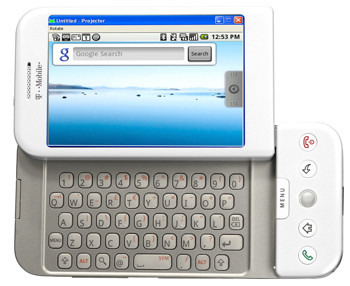
\includegraphics[height=8cm]{imagenes/capitulo2/htc-dream.jpg}
\caption{HTC Dream}
\end{figure} 


\section{Arquitectura}

Android es una plataforma para smartphones, pero ha evolucionado hacia otro tipo de dispositivos móviles como las tabletas. En el siguiente gráfico se muestra la estructura general de esta plataforma:
\begin{figure}[ht]
\centering
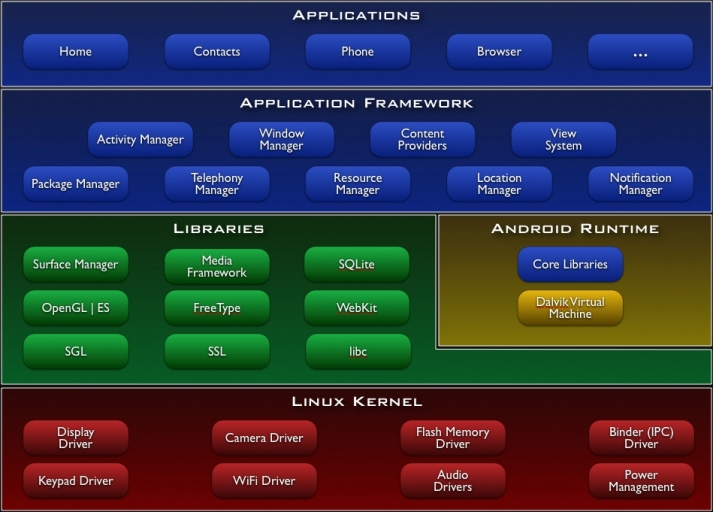
\includegraphics[height=9cm]{imagenes/capitulo2/androidArchitecture.jpg}
\caption{Arquiectura Android}
\end{figure} 

\begin{description}
\item [Un sistema operativo Linux,] responsable de gestionar los recursos ofrecidos por el hardware como memoria, batería, pantalla\ldots\ Cada fabricante ofrece distintos drivers para comunicarse con su hardware y es el sistema operativo quien nos independiza de tener que conocer cada una de ellas, 
ofreciéndonos una interfaz común. También es el responsable de gestionar los distintos recursos que ofrece el dispositivo como son:
\begin{multicols}{2}
\begin{itemize}
\item Pantalla
\item Teclado
\item Cámara de fotos
\item Wifi
\end{itemize}
\begin{itemize}
\item Memorias flash
\item Audio 
\item Batería
\item etc
\end{itemize}
\end{multicols}

\item [Librerías en C y C++] que permiten acceder al hardware del dispositivo móviles u otros componentes que estén integrados. Las librerías principales se listan a continuación:
\begin{itemize}
\item Surface Manager: gestiona los gráficos mostrados en pantalla.
\item Media Framework: permite reproducir imágenes, audio y vídeo. 
\item SQLite: gestiona el acceso a bases de datos relacionales. 
\item WebKit: navegador web optimizado.  
\item SGL: permite realizar gráficos en 2D.  
\item OpenGL ES: permite realizar gráficos en 3D.
\item FreeType: procesamiento de imágenes vectoriales.
\end{itemize}

\item [Entorno de ejecución,] con la máquina virtual basada en Java llamada \textbf{Dalvik}, que ha sido modificada para optimizar entornos con restricciones de procesamiento, memoria y espacio, como son los dispositivos móviles. 

Dalvik permite independizar las aplicaciones del hardware mediante ficheros con un formato con extensión \textbf{dex}, que significa Dalvik executable. 

El programador utilizará la sintaxis Java y dispondrá de un amplio conjunto de JME\footnote{Java Micro Edition: Librería Java para el desarrollo de aplicaciones móviles}, optimizado para Dalvik. Al compilar el código se generarán bytecode de java, que posteriormente es optimizado mediante la herramienta dx, para que optimice el código y genere el fichero dex. 

La comunicación del entorno de ejecución con las librerías en C y C++ se realiza mediante JNI\footnote{Java native interface: Interfaz nativo de java}.

\item [Framework de aplicaciones,] ofrece la funcionalidad básica de Android, siendo las más destacables:
\begin{itemize}
\item Activity Manager: gestiona las actividades que se están ejecutando en el smarthpone. Toda aplicación en Android está compuesta por actividades y se define como un componente gráfico con su propio ciclo de vida. En la siguiente sección veremos en detalle la composición las aplicaciones en Android.
\item Windows Manager: gestiona qué es lo que se visualiza por pantalla. Cuando una actividad necesita ser visualizada por el usuario, ha de invocar a este componente.
\item Contents Provider:  gestiona grupos de información que son utilizados por varias aplicaciones. Los principales contenidos de Android son la agenda de contactos y el calendario.
\item Telephony Manager: permite acceder a las funcionalidades de telefonía del dispositivo, protocolos de comunicación permitidos, los datos de la SIM, estado de la conexión\ldots
\item Resource Manager: permite acceder al contenido estático de la aplicación, como ficheros de audio, XML de configuración\ldots
\item Location Manager: permite acceder a la información de localización del dispositivo por GSP, WIFI y las torretas de telefonía.
\item Notification Manager: permite acceder al componente de notificaciones de Android, un panel donde se registran avisos de distinta índole, por ejemplo, nuevos mensajes, llamadas perdidas, actualizaciones\ldots
\end{itemize}

\item [Otras aplicaciones] son instaladas en el dispositivo por las compañías u los usuarios de los dispositivos móviles. La forma más común en la que estás aplicaciones pueden ser instaladas es desde la web de Google. Inicialmente surgió con el nombre de Google Market y posteriormente fue renombrado como Google Play. \begin{center}\texttt{https://play.google.com}\end{center}
\end{description}


\section{Entorno de desarrollo}

El siguiente paso, tras haber tomado conciencia sobre qué es Android, es explicar las herramientas principales que nos ofrece la plataforma para facilitar el desarrollo de aplicaciones:

\begin{description}
\item [Eclipse,] un IDE\footnote{Integrated developement Environment: aplicación compuesta por un conjunto de herramienta para el desarrollo de aplicaciones} desarrollado por la comunidad OpenSource, que se caracteriza por permitir ser configurado por terceros. 
\item [Android Developer Tools (ADT),] plugin que configura Eclipse para poder desarrollar aplicaciones en Android.
\item [Android Debug Bridge (ADB)] es una herramienta que permite conectarse vía USB con dispoistivos Android y realizar un conjunto de acciones sobre él. Las más utilizadas son instalar aplicaciones, mover ficheros o crear una sesión mediante el protocolo de telnet, accediendo directamente con el sistema operativo Unix del dispositivo móvil.
\item [Un emulador] que cubre gran parte de las características soportadas en dispositivos móviles con Android. Permite ejecutar aplicaciones sin necesidad de tener un dispositivo físico. 
\item [Android Virutal Device (ADV),] ficheros que definen la configuración hardware de un dispositivo móvil y son cargados en el emulador. Son generados mediante una herramienta llamada Android, integrada dentro de su entorno de desarrollo.
\item [Mksdcard,] herramienta que permite simular una tarjeta de memoria virtual sobre un fichero, la cual podrá cargarse dentro del emulador.
\item [Logcat,] herramienta que nos permite ver las trazas de información que van dejando todas las aplicaciones que se ejecutan en el dispositivo móvil.
\item [Otras herramientas] que permiten diversas funcionalidades para generar copias de seguridad, analizadores y ofuscadores de código\ldots\ 
\end{description}


\section{Estructura de una aplicación}

Una vez que tenemos montado nuestro entorno de desarrollo con las herramientas mencionadas en el apartado anterior, se explicará la estructura de una aplicación en Android. Al crear un proyecto, se generará la siguiente estructura de ficheros:
\begin{itemize}
\item \textbf{AndroidManifest.xml,} fichero principal de la aplicación donde se indican las características principales de la aplicación. Es obligatorio definir cuales son las actividades que componen la aplicación, cuál de ellas es la principal, la versión de la aplicación y versión requerida del SDK. Además se han de definir cuáles son los permisos necesarios para el correcto funcionamiento de la aplicación, por ejemplo envío automático de mensajes, acceso al GPS, contactos, cámara,  etc. Al instalar la aplicación, se indicará al usuario los permisos que requiere y ha de aceptarlos si desea instalarla.
\item Directorio  \textbf{src} donde se ubican las fuentes java. El proyecto creado con el plugin ADT, genera una clase llamada como el proyecto que extiende de Activity y será el punto inicial que se ejecutará en la aplicación.
\item Directorio \textbf{res} donde se ubican distintos recursos en una jerarquía de directorios en función de las características de los mismos:
\begin{itemize}
\item drawable-hdpi: contiene las imágenes de alta densidad.
\item drawable-mdpi: contiene las imágenes de media densidad
\item drawable-ldpi: contiene las imágenes de baja densidad.
\item layout: contiene ficheros xml con la definición de las interfaces gráficas que se cargarán en la actividad.
\item values: contiene ficheros xml donde se definen propiedades utilizadas por la aplicación como colores, cadenas de texto\ldots
\end{itemize}
\end{itemize}

Una aplicación Android puede estar compuesta por varias actividades, consideradas como unidades atómicas, buscando en ellas una alta cohesión y bajo acoplamiento. 
\newline 

Debido a las limitaciones del dispositivo móvil, las actividades son gestionadas por Android atendiendo a su estado y gestionarlas de la forma más eficiente posible.
\newline

Para comprender mejor el concepto de actividad, recurriremos al ejemplo principal de la página de desarrolladores de Android\footnote{http://developer.android.com}. El ejemplo \emph{Hello World} está compuesto por dos actividades, en la primera de ellas se solicita una cadena de texto y en la segunda se muestra la cadena con una letra mayor.  De forma coloquial, podemos entender las actividades como las distintas pantallas que componen una aplicación.

\begin{figure}[!h]
\centering
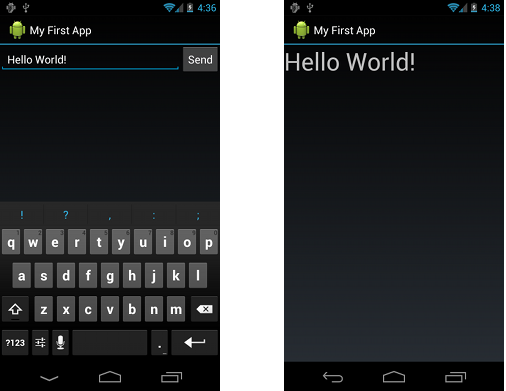
\includegraphics[height=8cm]{imagenes/capitulo2/firstapp.png}
\caption{Actividades del ejemplo Hello World}
\end{figure}

Toda actividad sigue un ciclo de vida, se van produciendo eventos que provocan una transición a un nuevo estado. Los eventos principales de este ciclo de vida son los siguientes:

\begin{itemize}
\item \textbf{onCreate:} Ocurre cuando la aplicación se crea. En este punto se ha de crear la interfaz gráfica e inicializar las estructuras de datos pertinentes.
\item \textbf{onStart:} Ocurre cuando la actividad se va a mostrar en pantalla por primera vez.
\item \textbf{onRestart:} Ocurre cuando la actividad parada va a mostrarse de nuevo.
\item \textbf{onResume:} La actividad comienza a visualizarse en pantalla, interactuando con el usuario.
\item \textbf{onPause:} La aplicación se ha pausado. Y deja de interaccionar con el usuario. En ese momento, todos los datos serán almacenados en la memoria secundaria, ya que el sistema puede terminar esta actividad pausada si se ve baja de recursos. Si se reactivara, pasaría al estado \texttt{onResume}.
\item \textbf{onStop:} Cuando una segunda actividad, nueva o reactivada, ha de mostrarse en pantalla. La actividad mostrada en esos momentos recibe este evento, pasando a un segundo plano, un estado candidato a ser destruido en caso de falta de memoria. Si la actividad pasase de nuevo al primer plano, cambiaría a estado \texttt{onRestart}.
\item \textbf{onDestroy:} La aplicación acaba y se destruye, bien porque acaba ella mima o el sistema la termina.
\end{itemize}

\begin{figure}[!h]
\centering
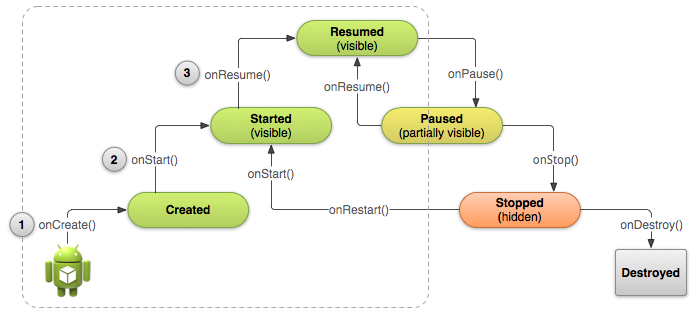
\includegraphics[height=5.8cm]{imagenes/capitulo2/activity_lifecycle2.png}
\caption{Ciclo de vida de una actividad}
\end{figure}

\section{Evolución}

Actualmente existen varias versiones de Android que van incorporando nuevas funcionalidades. La primera versión, llamada \textbf{Apple Pie} (Pastel de manzana), sólo se incorporo al modelo HTC-Dream\footnote{Para más información sobre las especificaciones hardware consulte los apéndices}.
\newline

Su característica más importante consistía en poder sincronizar los datos del móvil y la cuenta de Google. Otras  características a destacar son:
\begin{multicols}{2}
\begin{itemize}
\item HSDPA/850/900/1800/1900.
\item GPRS.
\item SMS y MMS.
\item Cámara de fotos.
\item Wifi (Cifrado WEP).
\item Bluetooth
\item USB 1.0
\item Navegador HTML 
\item Aplicación YouTube
\end{itemize}
\begin{itemize}
\item Aplicación música
\item Aplicación Android Market\footnote{Centro de descarga de aplicaciones para el móvil}
\item Aplicación de bloqueo táctil
\item Aplicación GMail
\item Aplicación Google Calendar
\item Aplicación Google Contacts
\item Aplicación Google Talk\footnote{Aplicación de intercambio de mensajes de texto}
\item Aplicación Google Maps

\end{itemize}
\end{multicols}

\begin{figure}[!h]
\centering
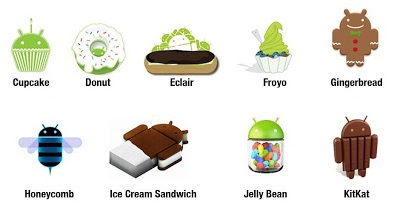
\includegraphics[width=13cm]{imagenes/capitulo2/android-versiones.jpg}
\caption{Logotipos de las versiones de Android}
\end{figure}
\subsection{Cupcake} 

El 30 de abril del 2009 se presenta la versión 1.5 de Android, conocida como Cupcake. Esta versión se caracteriza por:

\begin{itemize}
\item Estar basada en el kernel Linux 2.6.27.
\item Tener un teclado virtual, innecesario en la versión anterior ya que el HTC Dream tenía un teclado físico. 
\item Se mejora la velocidad de la cámara de fotos y se permite grabar vídeos.
\item Permite subir video y fotos a YouTube y Picassa.
\item Se mejorar el soporte bluetooth estéreo.
\item Se permite insertar nuevos widget desarrollados por terceros.
\item Transiciones de pantallas animadas.
\item Mejoras de tiempo de respuesta en el acceso GPS al utilizar A-GPS.
\item Mejorar el rendimiento en WebKit con el interprete de javascript \emph{SquirelFish}.
\item Posibilidad de cortar y pegar texto seleccionado.
\item Gestor de aplicaciones instaladas.
\end{itemize} 

\begin{figure}[!h]
	\centering	
	\subfloat[Teclado virtual]{
	          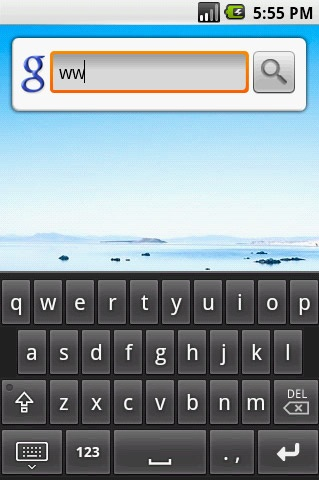
\includegraphics[height=7cm]{imagenes/capitulo2/cupcake-keyboard.jpg}
	}
	\hspace{0.8cm}
	\subfloat[Gestor de aplicaciones]{
	          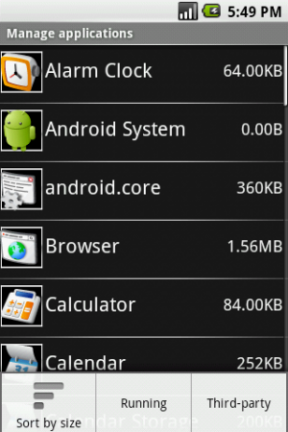
\includegraphics[height=7cm]{imagenes/capitulo2/cupcake-appmanager.png}
	}
	\caption{Novedades de la versión Cupcake}
\end{figure}


\subsection{Donut}

El 15 de Septiembre de 2009 se presenta la versión 1.6, conocida como Donut. Esta versión se caracteriza por:

\begin{itemize}
\item Soporte para telefonía de datos mediante CDMA.
\item Creación de redes virtuales mediante VPN.
\item Cifrado WAP en conexiones WiFi.
\item Motor de texto por voz que permite traducir un texto y escucharlo.
\item Nuevo applet de búsqueda que consulta tanto en Internet cómo en los datos del dispositivo.
\item Gestures que permite realizar acciones en el móvil al realizar una trazada con el dedo sobre la pantalla.
\item Soporte para pantallas de distintos tamaños y densidades.
\item Aplicación de gestión de batería por aplicación.
\end{itemize}

\begin{figure}[!h]
	\centering	
	\subfloat[Applet búsqueda]{
	          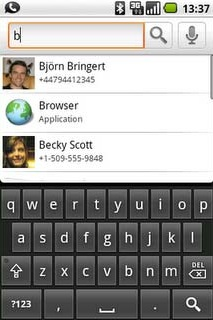
\includegraphics[height=7cm]{imagenes/capitulo2/donut-quicksearch.jpg}
	}
	\subfloat[Gestoures]{
	          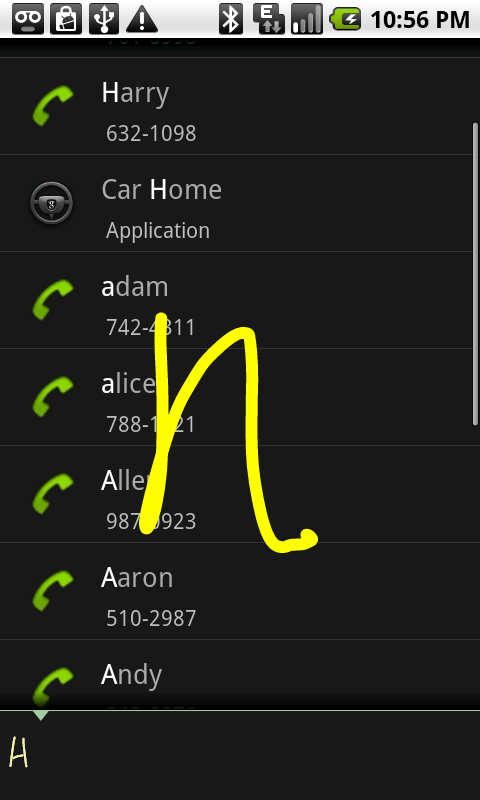
\includegraphics[height=7cm]{imagenes/capitulo2/donut-gestoures.png}
	}
	\subfloat[Gestor batería]{
	          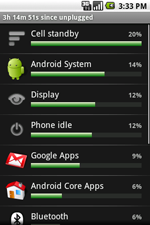
\includegraphics[height=7cm]{imagenes/capitulo2/donut-battery.png}
	}
	\caption{Novedades de la versión Donut}
\end{figure}

\subsection{Eclair} 

El 26 de octubre del 2009 se presenta la versión 2.0 de Android, conocida como Eclair. Esta versión se caracteriza por:

\begin{itemize}
\item Sincronización con Exchange.
\item Sincronización con multiples cuentas.
\item Soporte HTML 5.
\item Novedades en el uso de cámara que incluye flash, zoom digital\ldots
\end{itemize}

\subsection{Froyo} 

El 20 de mayo del 2010 se presenta la versión 2.2 de Android, conocida como Froyo. Esta versión se caracteriza por:
\begin{itemize}
\item Optimizaciones en velocidad,memoria y rendimiento.
\item Soporte Flash.
\item Instalación de aplicaciones en la SD en el almacenamiento interno de algunos dispositivos móviles.
\item Anclaje por USB, permitiendo al dispositivo al que se conecte el móvil usar la red de datos.
\item Soporte C2DM (Cloud to device Messaging) que permite sincronizar datos de una forma más efectiva. En vez de pooling es el servidor quien notifica al cliente que los datos han sido modificados.
\item Soporte OpenGL ES 2.0 para generación de gráficos tridimensionales.
\end{itemize}

\subsection{Gingerbread}

El 6 de diciembre del 2010 se presenta la versión 2.3 de Android, conocida como Gingerbread. Esta versión se caracteriza por:
\begin{itemize}
\item Aplicación Google Wallet para realizar pagos mediante móvil.
\item Soporte NFC (Near Field Communication). Esta tecnología permite comunicar de forma inalámbrica de corto alcance y alta frecuencia entre dispositivos para el intercambio de datos.
\item Soporte VoIP para realizar telefonía IP (Llamadas por Internet).
\item Mejora de rendimiento en el recolector de basura de Davilk.
\item Soporte nativos para sensores como el giroscopio y barómetro.
\end{itemize}

\begin{figure}[!h]
\centering
         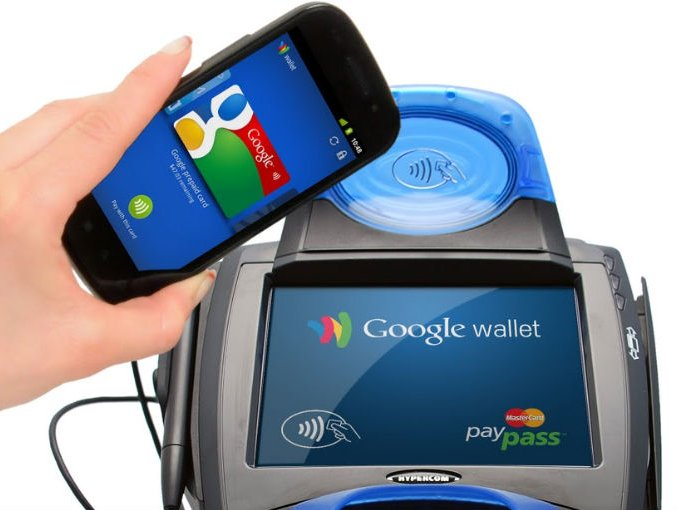
\includegraphics[height=6cm]{imagenes/capitulo2/gingerbreak-wallet.jpg}
	\caption{Google Wallet}
\end{figure}

\subsection{Honeycomb}

El 22 de febrero del 2011 se presenta la versión 3.0, conocida como Honeycomb. Esta versión consiste en una adaptación de la interfaz gráfica para tabletas. También se incluye un mayor soporte USB para conectar dispositivos a la tableta.

\begin{figure}[!h]
\centering
         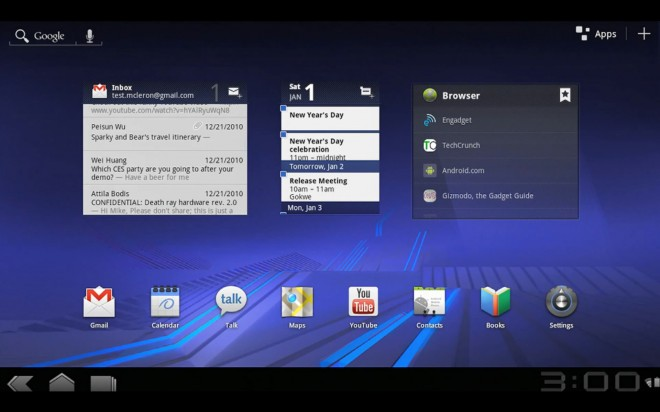
\includegraphics[width=10cm]{imagenes/capitulo2/honeycomb-screen.jpg}
	\caption{Nueva interfaz gráfica}
\end{figure}

\subsection{Ice Cream Sandwich}

El 19 de octubre del 2011 se presenta la versión 4.0 de Android, conocida como Ice Cream Sandwich. Esta versión unifica las dos anteriores, siendo tanto para móviles como para tabletas. Esta versión se caracteriza por:
\begin{itemize}
\item Se basa en el kernel 3.0.1 de Linux.
\item Soporte WiFi direct, que permite conectar dispositivos por WiFi sin necesidad de puntos de acceso.
\item Grabación de vídeos en FullHD.
\item Interfaz gráfica de usuario acelerada mediante hardware.
\item Aplicación Android Beam para intercambio de ficheros mediante NFC.
\item Desbloqueo facial.
\item Soporte para fotos panorámicas.
\item Barra multitarea que permite ver todas las aplicaciones activas.
\end{itemize}

\begin{figure}[!h]
	\centering	
	\subfloat[Nueva interfaz]{
	          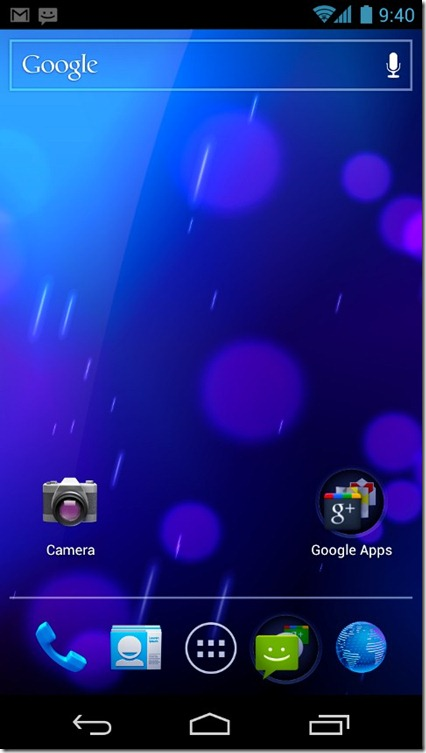
\includegraphics[height=7cm]{imagenes/capitulo2/ics-homescreen.jpg}
	}
	\hspace{0.8cm}
	\subfloat[Teclado deslizante]{
	          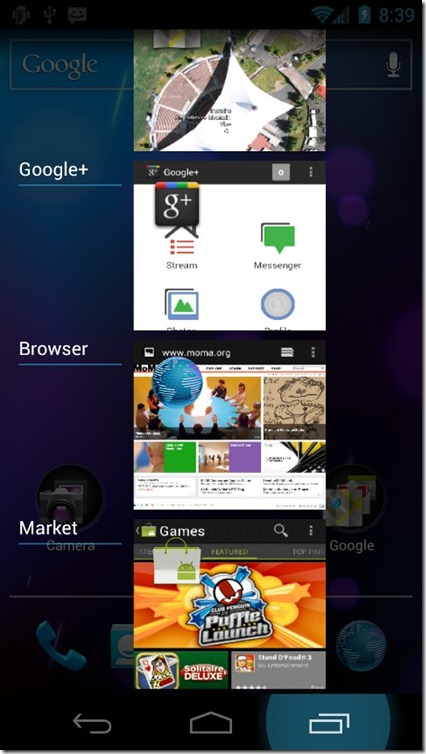
\includegraphics[height=7cm]{imagenes/capitulo2/ics-multitasking.jpg}
	}	
	\caption{Novedades de la versión Ice Cream Sandwich}
\end{figure}


\subsection{Jelly Bean}

El 9 de julio del 2012 se presenta la versión 4.1 de Android, conocida como Jelly Bean. Esta versión se caracteriza por:
\begin{itemize}
\item Mejora la interfaz, integrando el proyecto Butter, ofreciendo una sensación de fluidez mayor al manejar el dispositivo.
\item Agrega nuevas funcionalidades a la aplicación de la cámara. Las posibilidad de crear imágenes panorámicas en 360 grados es la más destacable.
\item Soporte multi-usuario.
\item Aplicación de inteligencia artificial, Google Now, la cúal responderá a algunas preguntas típicas relacionadas con el tiempo, eventos, vuelos, lugares, tráfico, resultados deportivos\ldots
\item Teclado predictivo deslizante.
\end{itemize}

\begin{figure}[!h]
	\centering	
	\subfloat[Nueva interfaz]{
	          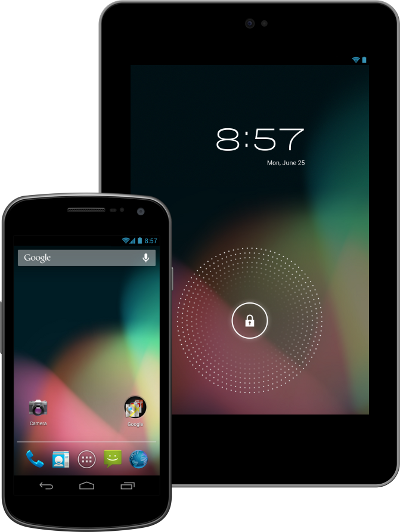
\includegraphics[height=6cm]{imagenes/capitulo2/jb-screenshot.png}
	}
	\hspace{0.8cm}
	\subfloat[Google Now]{
	          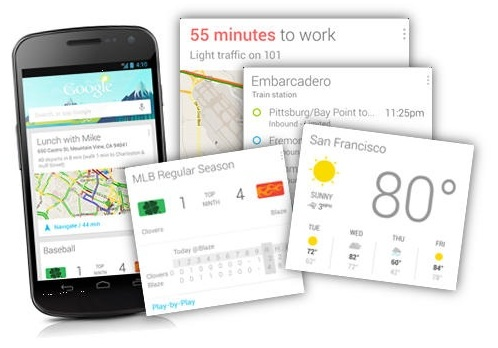
\includegraphics[height=6cm]{imagenes/capitulo2/jb-googlenow.jpg}
	}
	\caption{Novedades de la versión Jelly Bean}
\end{figure}


\subsection{Kit Kat}

Junto con el nuevo móvil de Google, el Nexus 5, el 31 de octubre de 2013 se presenta la versión 4.4 de Android, conocida como Kit Kat.  El objetivo principal de esta versión es resolver el problema de fragmetación de la plataforma, en la cual existe muchas versiones de Android. Para cubrir esta meta, se ha optimizado el uso de batería y la RAM, pudiendo ejecutarse en la mayoría de los móviles actuales.
